\documentclass{weekly}
\begin{document}
\maketitlew{Аналитическая механика}{1}{6}{23}

\begin{wrapfigure}{r}{.28\textwidth}
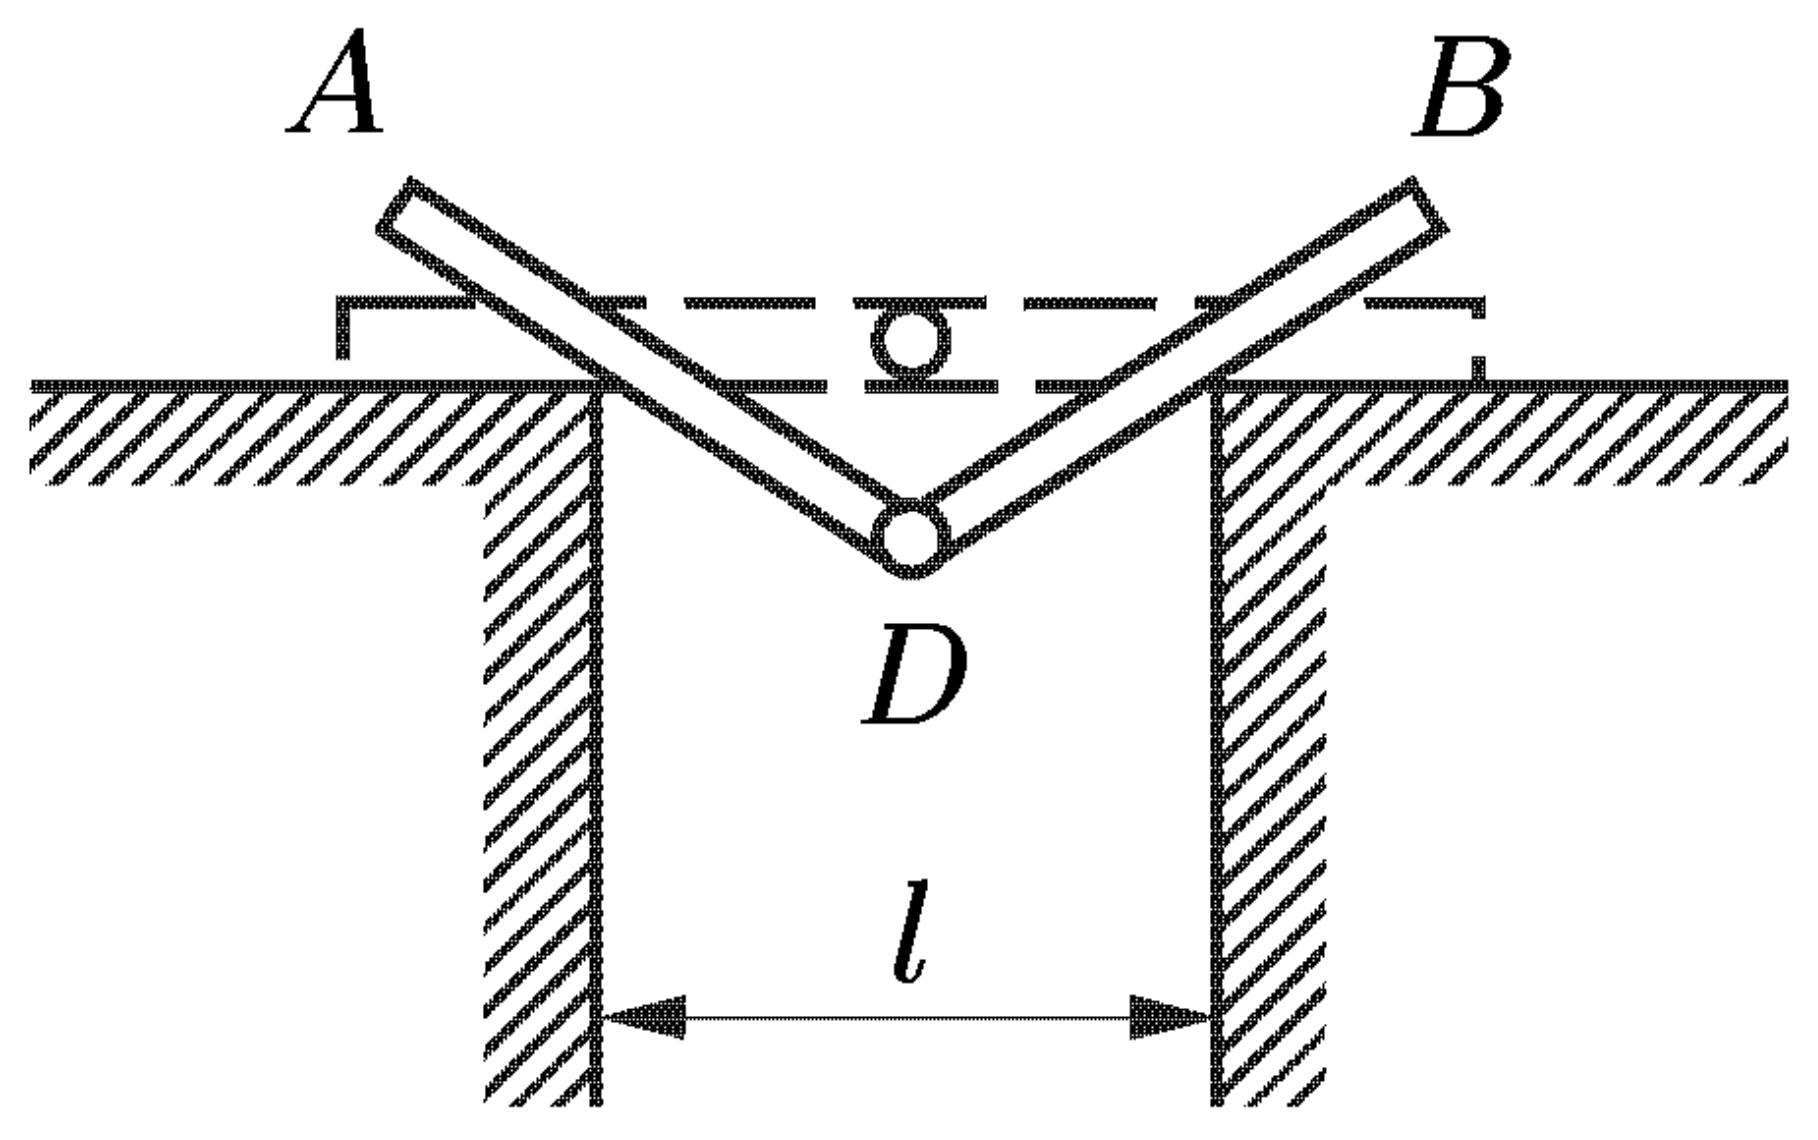
\includegraphics[width=\linewidth]{7-29}
\end{wrapfigure}
\paragraph{7.29.} Однородные стержни~$AD$ и~$BD$, шарнирно соединённые
в~точке~$D$, опираются на~два гладких угла. Длина каждого стержня
равна расстоянию между опорами~$l$. В~начальный момент стержни
горизонтальны и~расположены симметрично относительно опор,
а~затем (после малого начального толчка) приходят в~движение
за~счёт собственного веса, причём точка~$D$ перемещается по~вертикали.
Определить скорость точки~$D$ в~момент, когда концы стержней~$A$ и~$B$
достигнут угловых точек.

$\blacktriangleright$ При~решении задачи~3.12 было показано,
что~скорость~$v_T$ точки касания стержня вершины угла
направлена вдоль стержня и~связана со~скоростью точки~$D$
и~углом между стержнями~$\varphi$ соотношением
\begin{equation}
    v_T = v_D \cos\frac\varphi 2.
\end{equation}

Применив закон сохранения энергии и~теорему Кёнига, получим
для~рассматриваемого момента времени ($\varphi\to\varphi_0 = 60^\circ$):
\begin{equation}
    0 = -2 \cdot g\frac{l \cos\frac{\varphi_0}{2}}{2} +
            2 \cdot \frac{v_C^2}{2} +
            2 \cdot \frac{l^2}{12} \frac{\omega^2}{2}.
    \label{7.29:energy}
\end{equation}

$\triangleright$ Пусть концы~$\vec r_1$ и~$\vec r_2$ однородного стержня,
совершающего плоскопараллельное движение, имеют скорости~$\vec v_1$
и~$\vec v_2$. Найдём скорость~$\vec v_C$ его центра масс
и~угловую скорость~$\omega$:
\begin{align}
    \vec r_C = \dfrac{\vec r_1 + \vec r_2}{2}
&\then
    \vec v_C = \dfrac{\vec v_1 + \vec v_2}{2};
\\
    \vec v_2 - \vec v_1 = \vec\omega \times (\vec r_2 - \vec r_1)
&\then
    \vec\omega \times (\vec v_2 - \vec v_1)
        = -\omega^2 (\vec r_2 - \vec r_1).
\end{align}
Последнее соотношение скаляризируем как
\begin{equation}
    \omega = \frac{\abs{v_2^{\perp} - v_1^{\perp}}}{l},
\end{equation}
что, в~общем-то, и~так было понятно. \hfill $\triangleleft$

Выполним соответствующие подстановки в~\eqref{7.29:energy}:
\begin{gather}
    \frac{\sqrt{3}}{2} gl = v_C^2 + \frac{1}{3} \omega^2 l^2
        = \left(v_T^2 + \frac{1}{4} \omega^2 l^2\right)
            + \frac{1}{12} \omega^2 l^2
        = v_D^2 \left(\cos^2\frac{\varphi_0}{2}
            + \frac{1}{3} \sin^2\frac{\varphi_0}{2}\right).
\end{gather}
\textbf{Ответ:}\qquad $v_D = \sqrt{\dfrac{3\sqrt{3}}{5}}$.
\hfill $\blacktriangleleft$

\bigskip
\begin{small}
\textsl{Примечание.} Вообще говоря, стержни оторвутся от~углов
раньше рассматриваемого момента времени.
Доказывать это утверждение здесь и~сейчас я, конечно же, не~буду.
\end{small}


\begin{wrapfigure}[6]{r}{.42\textwidth}
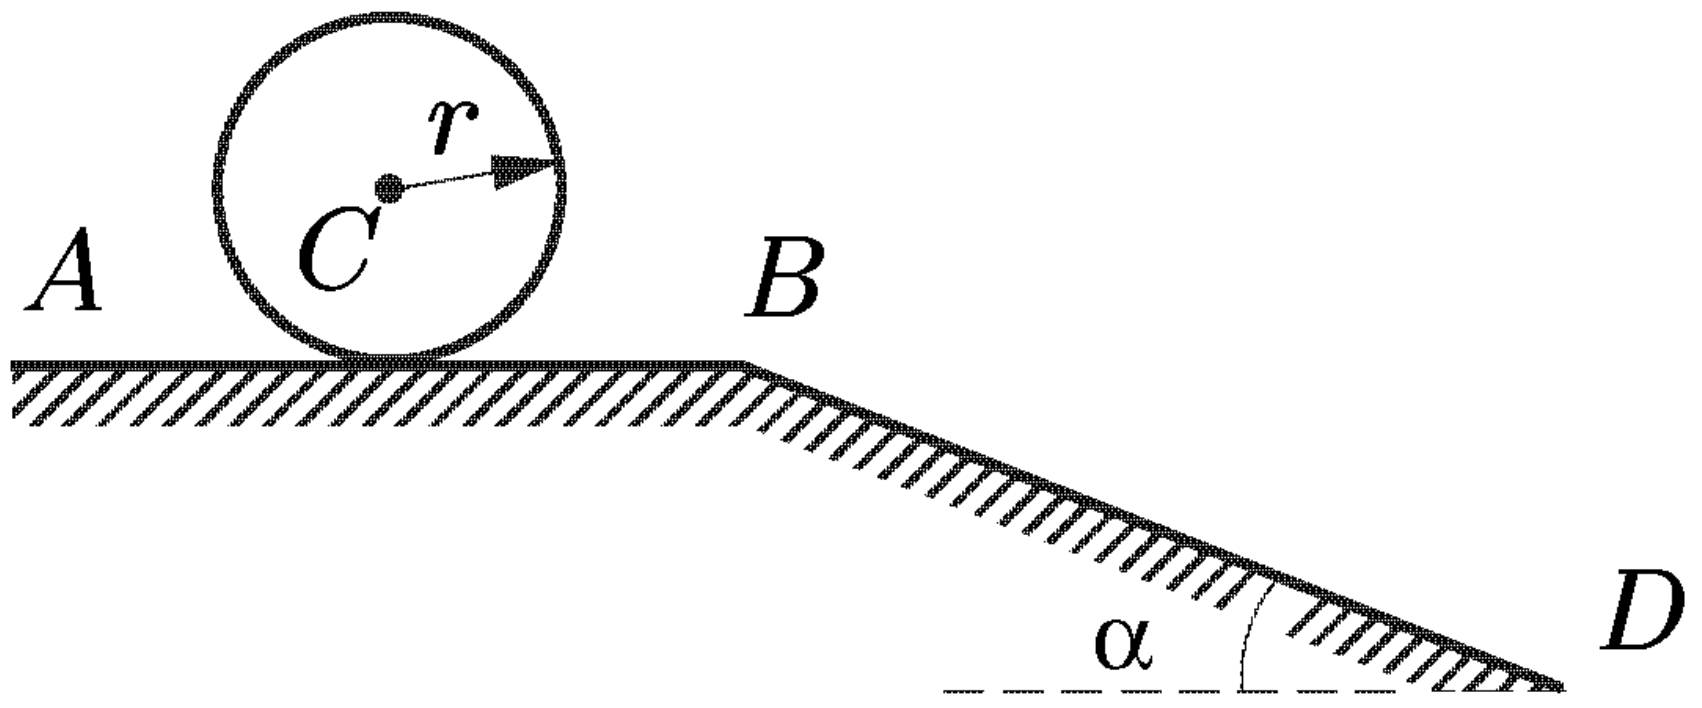
\includegraphics[width=\linewidth]{7-42}
\end{wrapfigure}
\paragraph{7.42.} Шар радиуса~$r$ катится без~проскальзывания
по~горизонтальной плоскости~$AB$, переходя с~этой плоскости
на~плоскость~$BD$, образующую угол~$\alpha$ с~горизонтом.
Достигнув точки~$B$, шар начинает поворачиваться вокруг неё.
В~начальный момент времени скорость центра~$C$ шара равна~$v_0$.
Найти наибольшее значение угла~$\alpha$, при~котором шар,
переходя на~наклонную плоскость, не~будет делать скачка.
(Отрыв шара происходит в~тот момент, когда проекция силы реакции
опоры в~угловой точки на~нормаль к~траектории шара обращается в~нуль.)

$\blacktriangleright$ Рассмотрим момент времени, когда
линия~$BC$ образует с~вертикалью угол~$\beta$.
Угловую скорость шара в~этот момент найдём из~ЗСЭ:
\begin{align}
    \frac{I_B}{2} \omega^2 = mgR(1-\cos\beta) +
            \frac{I_B}{2} \left(\frac{v_0}{R}\right)^2&, \\
    где~I_B &= \frac{2}{5}mR^2 + mR^2 = \frac{7}{5}mR^2.
\end{align}
Закон движения шара (в~проекции на~нормаль к~траектории центра)
запишется в~виде
\begin{equation}
    mg\cos\beta - R_N = m\omega^2 R
        = m\frac{v_0^2}{R} + \frac{10mg}{7} (1-\cos\beta).
\end{equation}
Нетрудно видеть, что~силу~$R_N$ можно обратить в~нуль:
\begin{equation}
    \cos\beta_0 = \frac{\frac{7v_0^2}{gR} + 10}{17}.
\end{equation}
Геометрическое ограничение~$\beta_0 \geqslant \alpha$
является искомым.

\medskip
\textbf{Ответ:}\qquad $\alpha_{\max} =
\arccos \left( \dfrac{7v_0^2}{17gR} + \dfrac{10}{17} \right)$.
\hfill $\blacktriangleleft$


\begin{wrapfigure}{r}{.23\textwidth}\vspace{-5mm}
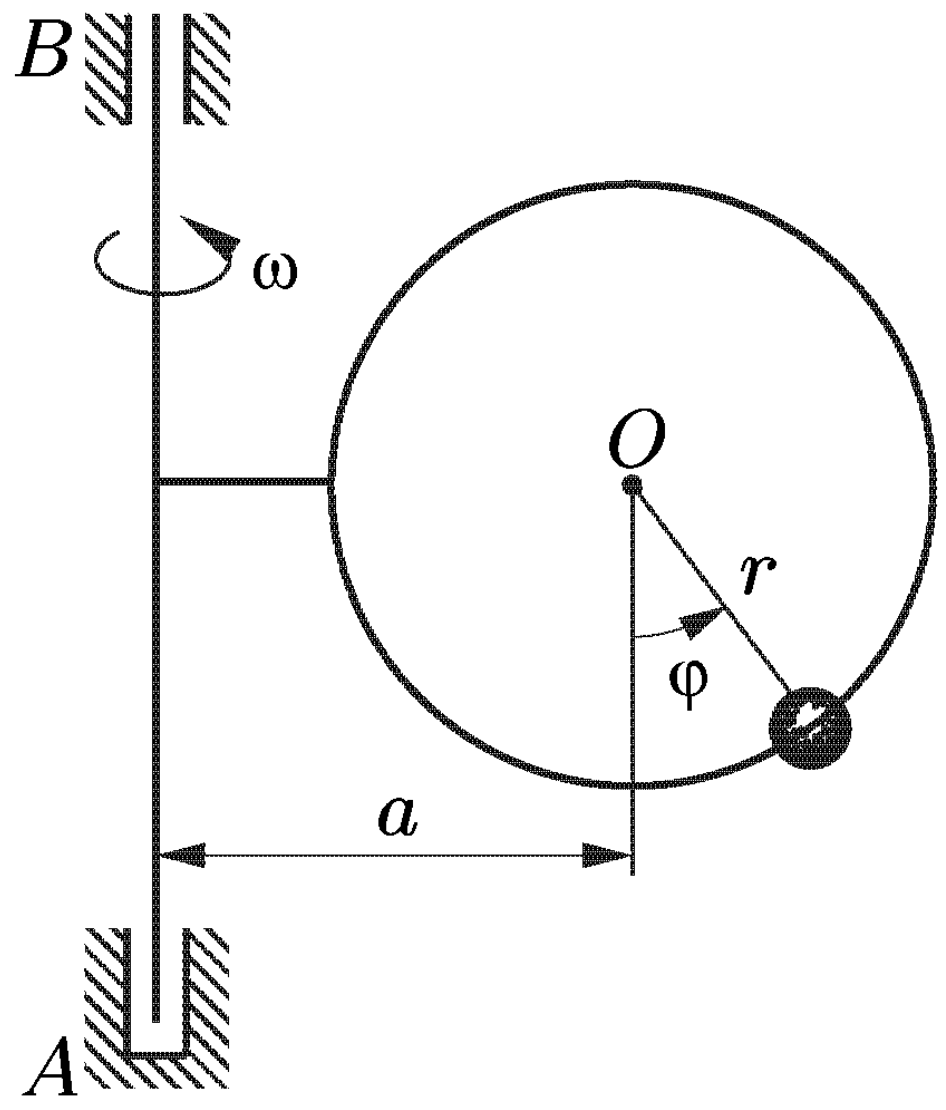
\includegraphics[width=\linewidth]{9-5}
\end{wrapfigure}
\paragraph{9.5.} Гладкое кольцо радиуса~$r$, плоскость которого
вертикальна, вращается с~постоянной угловой скоростью вокруг
вертикальной оси~$AB$, находящейся на~расстоянии~$a$
от~центра кольца~$O$. По~кольцу может скользить тяжёлая бусинка.
Найти угловую скорость, при~которой положение относительного
равновесия бусинки будет определяться заданным углом~$\varphi_0$,
если $a + r\sin\varphi_0 \neq 0$. Найти относительную скорость
бусинки в~зависимости от~угла~$\varphi$, если в~начальный момент
её скорость относительно кольца была равна нулю,
а~угол~$\varphi(0) = \varphi_0$.

$\blacktriangleright$ Равнодействующая центробежной и~гравитационной
сил должна быть направлена по~нормали к~кольцу, иначе равновесия
не~получится:
\begin{equation}
    \tan\varphi_0 = \omega^2(a + r\sin\varphi_0)/g.
\end{equation}

Во~вращающейся вместе с~кольцом системе отсчёта действуют
силовые поля гравитации и~инерции с~потенциалами
\begin{equation}
    u_g = -gr\cos\varphi; \quad
    u_c = -\omega^2 (a + r\sin\varphi)^2/2.
\end{equation}

\textbf{Ответ:}\qquad
$\omega = \sqrt{\dfrac{g \tan\varphi_0}{a + r\sin\varphi_0}}$; \quad
$v = \sqrt{2} \sqrt{u_g(\varphi_0) - u_g(\varphi)
    + u_c(\varphi_0) - u_c(\varphi)}$.
\hfill $\blacktriangleleft$


\begin{wrapfigure}{r}{.23\textwidth}
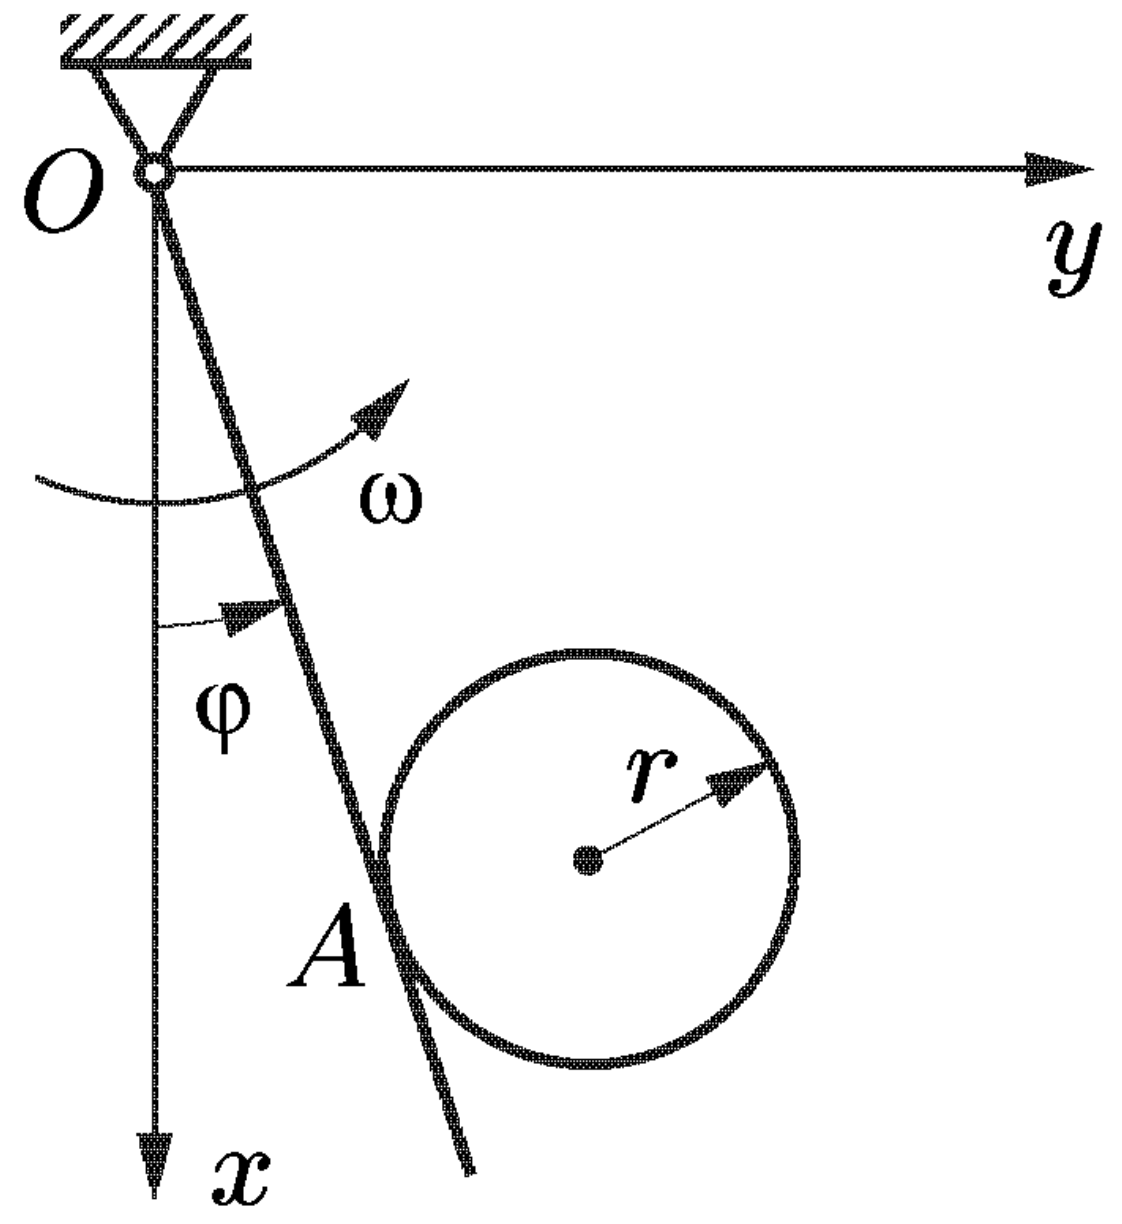
\includegraphics[width=\linewidth]{9-16}
\end{wrapfigure}
\paragraph{9.16.} Невесомый стержень, конец~$O$ которого
шарнирно закреплён, вращается с~постоянной угловой скоростью~$\omega$
вокруг горизонтальной оси~$Oz$, перпендикулярной плоскости рисунка.
По~стержню катится без~проскальзывания диск радиуса~$r$ и~массы~$m$.
Найти силу трения и~силу нормальной реакции со~стороны стержня
на~диск в~зависимости от~угла~$\varphi$ поворота стержня
и~расстояния~$l$ от~точки~$O$ до~точки~$A$ касания диска со~стержнем.
В~начальный момент точки~$O$ и~$A$ совпадали, а~диск покоился
относительно стержня.

$\blacktriangleright$ В~неинерциальной системе отсчёта, связанной
со~стержнем, к~центру диска приложены силы инерции:
центробежная, направленная от~точки~$O$, $m\omega^2\sqrt{l^2 + r^2}$,
и~кориолисова, направленная нормально~к~стержню.

Запишем для~диска теорему о~движении центра масс
в~проекциях на~направление стержня и~теорему об~изменении
кинетического момента диска с~учётом~$\varepsilon = \dot v/r$:
\begin{gather}
    m\dot v = m\omega^2 l + mg\cos\varphi - F_{тр};
        \label{9.16:Newt} \\
    \frac{mr^2}{2} \frac{\dot v}{r} = F_{тр} r
        \then m\dot v = 2F_{тр}.
        \label{9.16:rot}
\end{gather}
Подставляя результат из~\eqref{9.16:rot} в~\eqref{9.16:Newt},
сразу получаем ответ для~$F_{тр}$.

Аналогично, записывая уравнение для~проекций сил на~нормальное
к~стержню направление, имеем
\begin{equation}
    N = mg\sin\varphi + 2m\omega v - m\omega^2 r.
\end{equation}
Нахождение~$v$ в~таком случае представляет собой важнейшую задачу
народного хозяйства. Обозрим поля гравитационных и~центробежных сил
и~используем закон сохранения энергии:
\begin{equation}
    \frac12 mv^2 + \frac12 \frac{mr^2}{2} \frac{v^2}{r^2} =
        \frac34 mv^2 = mgl\cos\varphi + m\frac{\omega^2 l^2}{2}.
\end{equation}

\textbf{Ответ:}\qquad
$F_{тр} = \dfrac{m}{3} \left(\omega^2 l + g\cos\varphi\right)$; \quad
$N = mg\sin\varphi + \dfrac{4m\omega}{\sqrt{3}} \sqrt{gl\cos\varphi
    + \dfrac{\omega^2 l^2}{2}} - m\omega^2 r$.
\hfill $\blacktriangleleft$


\paragraph{9.24.} Однородный диск может катиться без~проскальзывания
по~горизонтальной направляющей~$Ox$, вращающейся с~постоянной
угловой скоростью~$\omega$ вокруг вертикальной оси~$Oy$.
Найти закон относительного движения диска.

$\blacktriangleright$ Запишем для~диска теорему о~движении центра масс
в~проекциях на~направляющую и~теорему об~изменении
кинетического момента диска с~учётом~$\varepsilon = \dot v/r$:
\begin{gather}
    m\dot v = m\omega^2 x - F_{тр}; \\
    \frac{mr^2}{2} \frac{\dot v}{r} = F_{тр} r.
\end{gather}
В~итоге имеем уравнение на~координату~$x$:
\begin{equation}
    \ddot x = \frac23 \omega^2 x.
\end{equation}

\textbf{Ответ:}\qquad
$x(t) = A \exp\left(+\sqrt{\dfrac23} \omega t\right)
+ B \exp\left(-\sqrt{\dfrac23} \omega t\right)$, \quad
$A, B \in \mathbb{R}$.
\hfill $\blacktriangleleft$


\begin{wrapfigure}[5]{r}{.15\textwidth}
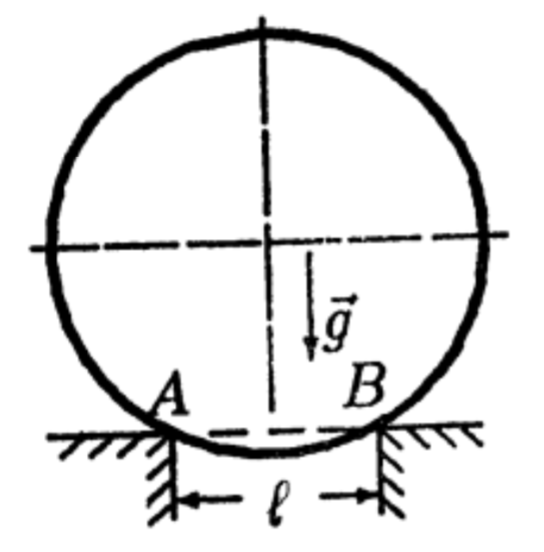
\includegraphics[width=\linewidth]{T1}
\end{wrapfigure}
\paragraph{T1.} Гладкий однородный цилиндр массы~$m$ и~радиуса~$r$
опирается на~расположенные на~одном уровне уступы~$A$ и~$B$,
расстояние между которыми равно~$l$. Определить реакцию опоры~$A$
в~момент удаления опоры~$B$ и~вертикальное смещение центра цилиндра
в~момент его отделения от~опоры~$A$.

$\blacktriangleright$ До~отрыва цилиндр движется по~окружности
с~центром в~$A$. Пусть в~некоторый момент времени линия
$AO$ ($O$~--- центр цилиндра) образует с~вертикалью угол~$\varphi$:
\begin{equation}
    m\frac{v^2}{r} = mg\cos\varphi - N.
\end{equation}
В~момент отрыва~$N = 0$, следовательно, $v_1^2 = gr\cos\varphi_1$.
Кроме того, из~закона сохранения энергии
\begin{equation}
    \frac{v_1^2}{r} = 2g(\cos\varphi_0 - \cos\varphi_1)
        \then \cos\varphi_1 = \frac23 \cos\varphi_0.
\end{equation}
Осталось разобраться с~геометрией:
\begin{gather}
    \cos\varphi_0 = \sqrt{1 - \left(\frac{l}{2r}\right)^2}; \\
    \Delta h = r(\cos\varphi_0 - \cos\varphi_1)
        = \frac{r \cos\varphi_0}{3}.
\end{gather}
\textbf{Ответ:}\qquad
$N_0 = mg \sqrt{1 - \left(\dfrac{l}{2r}\right)^2}$; \quad
$\Delta h = \dfrac{r}{3} \sqrt{1 - \left(\dfrac{l}{2r}\right)^2}$.
\hfill $\blacktriangleleft$

\end{document}
